\subsection{Get true energy of saturated electron}
\label{get_true_energy}
\subsubsection{Method}
Here we use the MVA BDTG (Gradient Boost) method which is the variants of BDT (Boosted
Decision Tree) to get the correct energy of saturated electron. The training target defined as:
\begin{eqnarray}
  T & = & log(\frac{E_{MC}}{E_{rawSC}}) \label{equ:target}
\end{eqnarray}
where the $E_{MC}$ is the true energy of electron and $E_{rawSC}$ is the raw
SuperCluster energy.
The training input variables are listed below:
\begin{itemize}
\item $E_{rawSC}$ : raw energy of the SuperCluster
\item $\frac{E_{max}}{E_{rawSC}}$ : energy of the most energetic crystal in the SC normalized to $E_{rawSC}$
\item $\frac{E_{3\times3}}{E_{rawSC}}$ : energy of the $3\times3$ matrix centered around the seed normalized to $E_{rawSC}$
\item $\frac{E_{5\times5}}{E_{rawSC}}$ : energy of the $5\times5$ matrix centered around the seed normalized to $E_{rawSC}$
\item $\frac{E_{left}}{E_{rawSC}}, \frac{E_{right}}{E_{rawSC}}, \frac{E_{top}}{E_{rawSC}}, \frac{E_{bottom}}{E_{rawSC}}$ : energy of the four crystals around the seed normalized to $E_{rawSC}$
\item $\frac{E_{2\times5~ left}}{E_{rawSC}}, \frac{E_{2\times5~ right}}{E_{rawSC}}, \frac{E_{2\times5~top}}{E_{rawSC}}, \frac{E_{2\times5~ bottom}}{E_{rawSC}}$ : energy of the four $2\times5$ crystal dominoes around the seed belonging to the $5\times5$ matrix normalized to $E_{rawSC}$
\item $\frac{E_{1\times5~ max}}{E_{rawSC}}$ : energy of the most energetic $1\times5$ domino belonging to the $5\times5$ matrix normalized to $E_{rawSC}$
\item $\frac{E_{preShower}}{E_{rawSC}}$ : energy measured in the PreShower normalized to $E_{rawSC}$ (only for endcap electrons)
\item $\eta$ and $\phi$ of the SC
\item $\eta$ and $\phi$ width of the SC
\item $i_{\eta}$ and $i_{\phi}$ of the SC seed
\item $\frac{H}{E}$
\item $\rho$
\end{itemize}

The configuration of the training and testing sample is \texttt{factory->PrepareTrainingAndTestTree\\("","nTrain\_Regression=0:nTest\_Regression=0:SplitMode=Random:NormMode=\\NumEvents:!V")} which means the the sample is split in half for training and testing, the events are selected randomly and the weight is one.
The configuration of the BDTG method is \texttt{factory->BookMethod(MVA::Types::kBDT, "BDTG","!H:!V:NTrees=1000::\\BoostType=Grad:Shrinkage=0.1:UseBaggedBoost:BaggedSampleFraction=0.5:\\nCuts=5:MaxDepth=3")}

The training target and input variables are the same with diphoton analysis in ref. \cite{CMS_AN_2015-241}. The electrons for the training are mc matched ($\Delta R ~<~0.1$) saturated electrons with mc energy less than 10 TeV and the $\eta$ ranges for the training are barrel and endcap separately.

\subsubsection{Sample}
The training and testing sample used is \texttt{/DoubleElectron\_FlatPt-300To6500/\\RunIISpring16DR80-PUFlat0to50\_80X\_mcRun2\_asymptotic\_2016\_v3-v1/AODSIM} \\ which is flat in pseudorapidity $\eta$ and transverse momentum $P_{T}$ in range 0.3 to 6.5 TeV. The distributions of $P_{T}$ and energy of generated electron versus $\eta$ are shown in Figure \ref{fig:Ptmc_Emc_eta}, one can see it is almost flat in $\eta$ and $P_{T}$ as expected. Besides, in Figure \ref{fig:Ptmc_Emc_eta} one can see the threshold energy for electron being saturated in barrel is around 2 TeV, while in endcap the threshold is not a consant which increases with the $\eta$. More details can be seen in Figure \ref{fig:Emax_eta} which is the distribution of $E_{max}$ versus $\eta$ for unsaturated and saturated electron, one can see the $E_{max}$ for saturated electron in barrel is almost flat while for endcap it is increase with $\eta$, the reason why $E_{max}$ will increase with $\eta$ in endcap for saturated electron maybe because of the "darkness" of crystal increase with $\eta$ in endcap.
Moreover from Figure \ref{fig:EmaxE24_Esc} we know $E_{sc}~ = ~E_{max}~+~E_{24}$ is correct also for saturated electron. From Figure \ref{fig:Esc_Emc} which gives the distributions of $E_{24}$, $E_{max}$, $E_{sc}$ versus generated energy $E_{mc}$ for saturated electron and the plots of $E_{sc}$ versus $E_{mc}$ should be equal to plots of $E_{24}$ versus $E_{mc}$ add the plots of $E_{max}$ versus $E_{mc}$. In addition, the saturated fraction of electron for different energy is shown in Figure \ref{fig:S_Fraction}, one can see there are a sharp turnon curve for barrel while for endcap it is gentle. Finally the number (or its fraction) of saturated crystal in $3\times3$ matrix with seed crystal in the center for different mc energy is shown in Figure \ref{fig:N_S_Emc}, one can see the fraction of having two saturated crystals is increase with the mc energy especially in barrel and the strange behaviour around the highest mc energy in barrel is because of the electrons which are very close to the gap.

\begin{figure}[bh]
  \begin{center}
    \begin{tabular}{cc}
      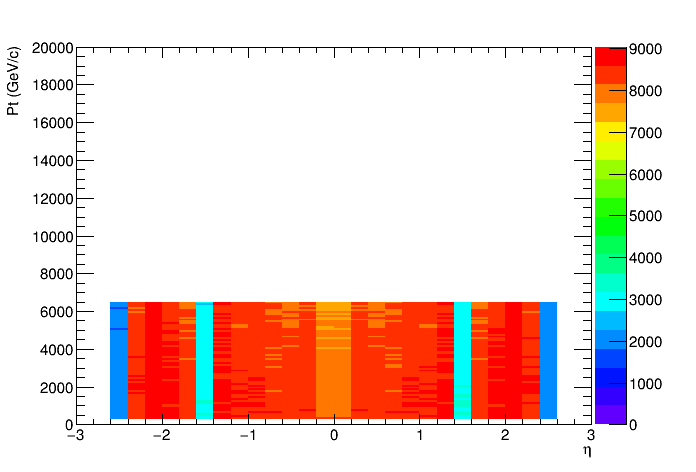
\includegraphics[width=0.45\textwidth]{chapters/Zprime/Saturation/images/FlatPt/Sample_variables/Ptmc_eta.png} &
      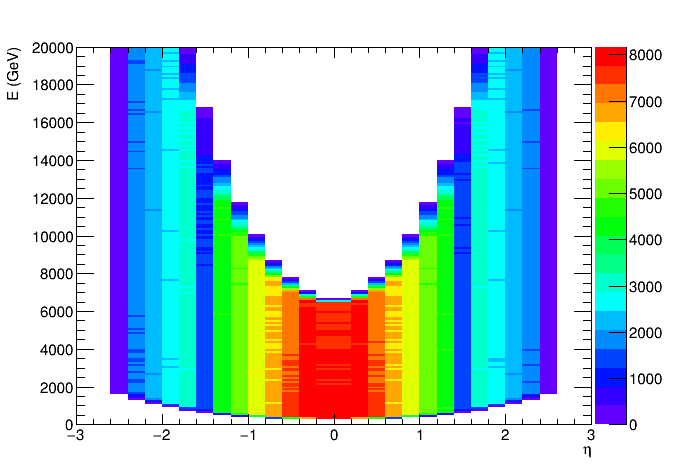
\includegraphics[width=0.45\textwidth]{chapters/Zprime/Saturation/images/FlatPt/Sample_variables/Emc_eta.png} \\
      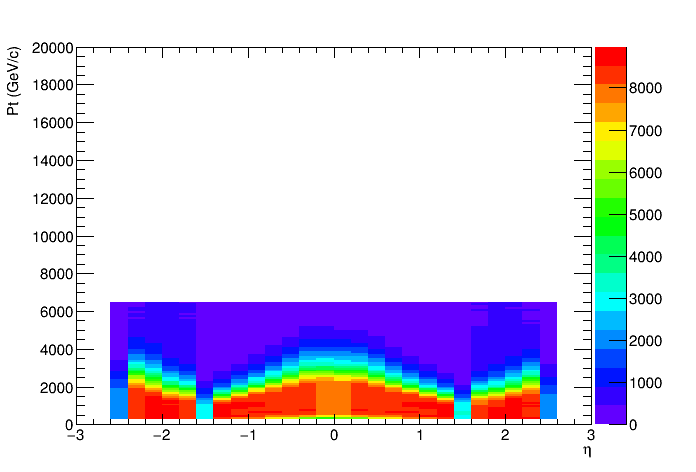
\includegraphics[width=0.45\textwidth]{chapters/Zprime/Saturation/images/FlatPt/Sample_variables/Ptmc_eta_nos.png} &
      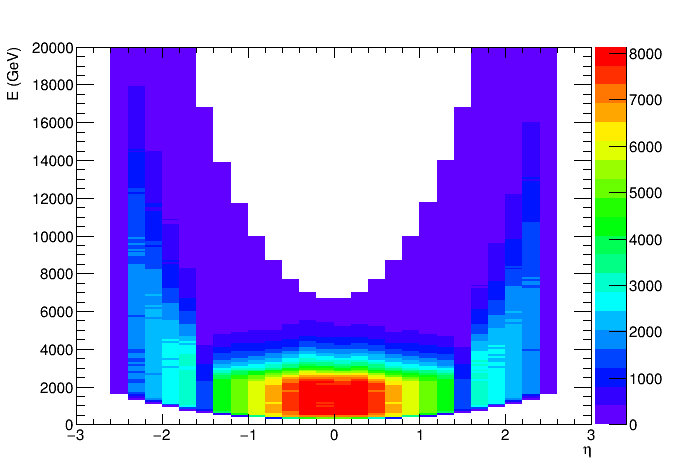
\includegraphics[width=0.45\textwidth]{chapters/Zprime/Saturation/images/FlatPt/Sample_variables/Emc_eta_nos.png} \\
      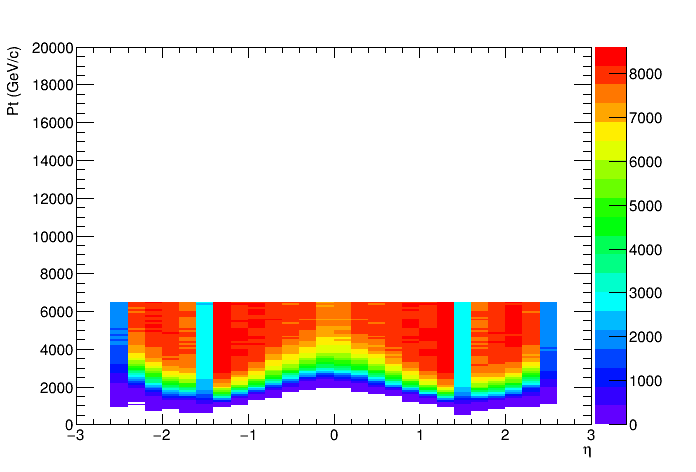
\includegraphics[width=0.45\textwidth]{chapters/Zprime/Saturation/images/FlatPt/Sample_variables/Ptmc_eta_s.png} &
      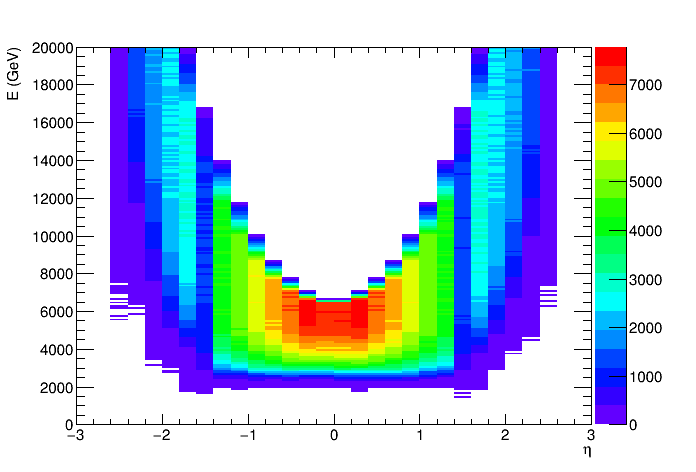
\includegraphics[width=0.45\textwidth]{chapters/Zprime/Saturation/images/FlatPt/Sample_variables/Emc_eta_s.png} \\
    \end{tabular}
    \caption{The distributions of $P_{T}$ for generated electrons versus $\eta$ (left) and energy of generated electrons versus $\eta$ (right) for all electrons (top), unsaturated electrons (middle) and saturated electrons (bottom).}
    \label{fig:Ptmc_Emc_eta}
  \end{center}
\end{figure}


\begin{figure}[bh]
  \begin{center}
    \begin{tabular}{cc}
      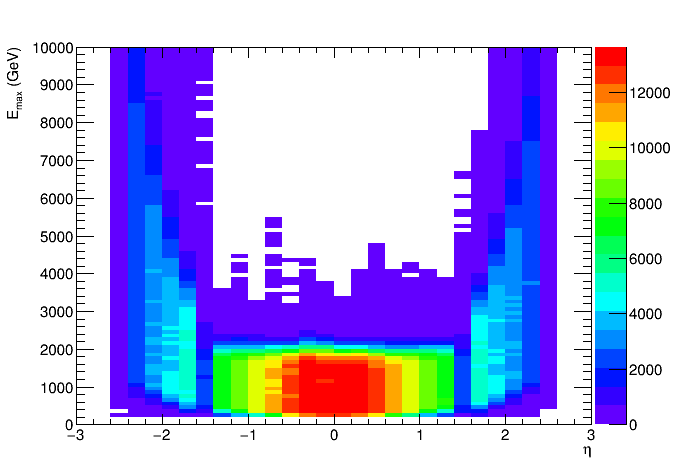
\includegraphics[width=0.45\textwidth]{chapters/Zprime/Saturation/images/FlatPt/Sample_variables/Emax_eta_nos.png} &
      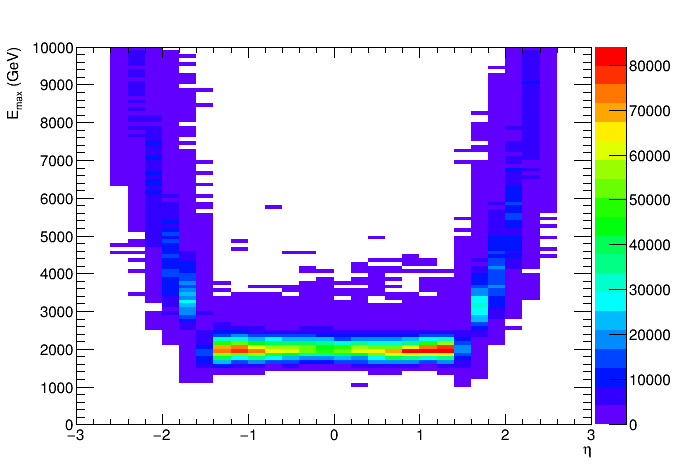
\includegraphics[width=0.45\textwidth]{chapters/Zprime/Saturation/images/FlatPt/Sample_variables/Emax_eta_s.png} \\
    \end{tabular}
    \caption{The distributions of $E_{max}$ versus $\eta$ for unsaturated electrons (left) and saturated electrons (right).}
    \label{fig:Emax_eta}
  \end{center}
\end{figure}


\begin{figure}[bh]
  \begin{center}
    \begin{tabular}{cc}
      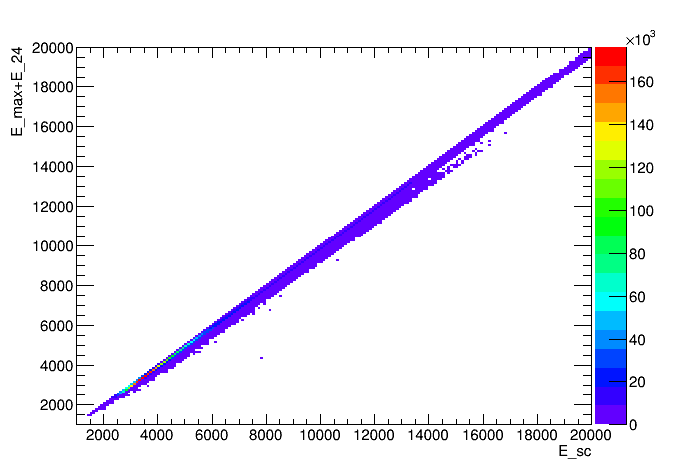
\includegraphics[width=0.45\textwidth]{chapters/Zprime/Saturation/images/FlatPt/Sample_variables/Esc_EmaxE24.png}
    \end{tabular}
    \caption{The distribution of $E_{max}~ + ~E_{24}$ versus $E_{sc}$ for saturated electrons.}
    \label{fig:EmaxE24_Esc}
  \end{center}
\end{figure}

\begin{figure}[bh]
  \begin{center}
    \begin{tabular}{cc}
      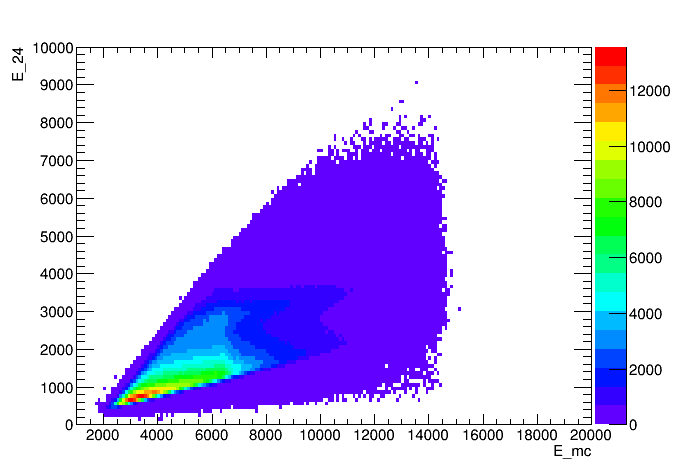
\includegraphics[width=0.45\textwidth]{chapters/Zprime/Saturation/images/FlatPt/Sample_variables/Emc_E24_Barrel.png} &
      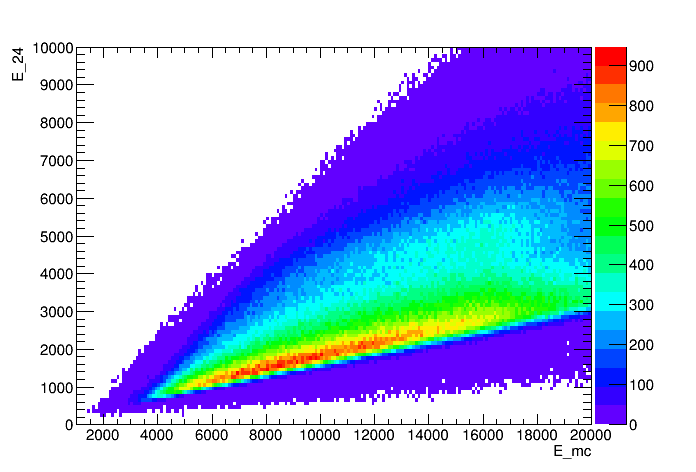
\includegraphics[width=0.45\textwidth]{chapters/Zprime/Saturation/images/FlatPt/Sample_variables/Emc_E24_Endcap.png} \\
      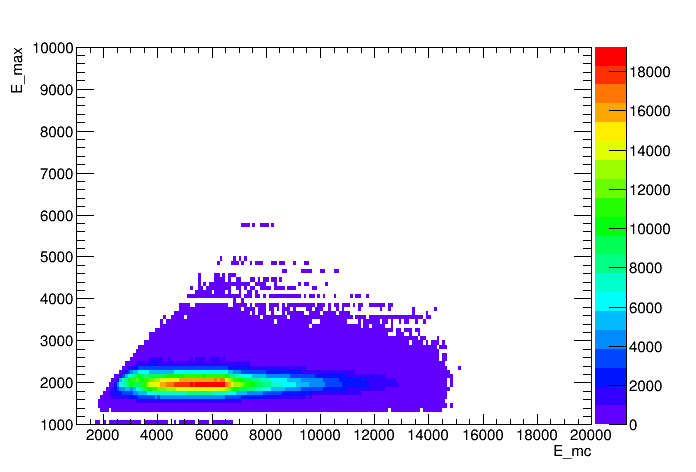
\includegraphics[width=0.45\textwidth]{chapters/Zprime/Saturation/images/FlatPt/Sample_variables/Emc_Emax_Barrel.png} &
      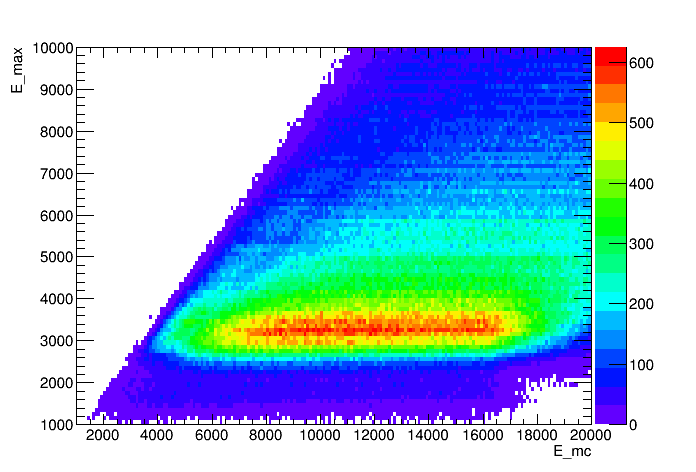
\includegraphics[width=0.45\textwidth]{chapters/Zprime/Saturation/images/FlatPt/Sample_variables/Emc_Emax_Endcap.png} \\
      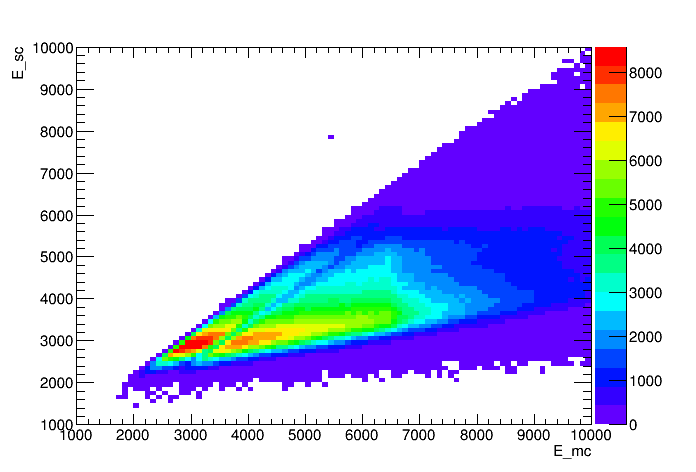
\includegraphics[width=0.45\textwidth]{chapters/Zprime/Saturation/images/FlatPt/Sample_variables/Emc_Esc_Barrel.png} &
      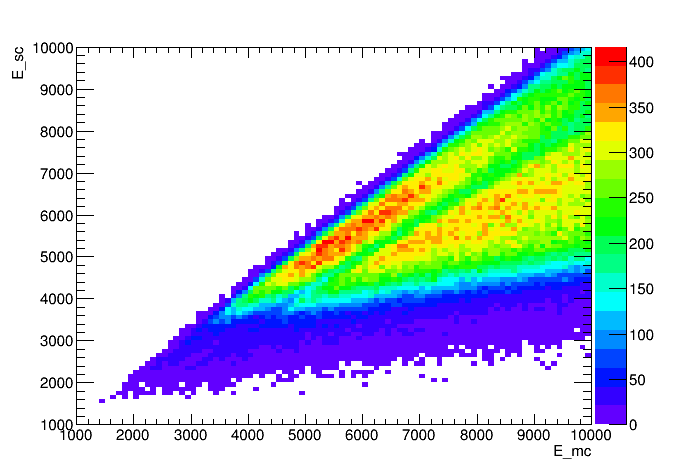
\includegraphics[width=0.45\textwidth]{chapters/Zprime/Saturation/images/FlatPt/Sample_variables/Emc_Esc_Endcap.png} \\
    \end{tabular}
    \caption{The distributions of $E_{24}$ versus $E_{mc}$ (top), $E_{max}$ versus $E_{mc}$ (middle) and $E_{sc}$ versus $E_{mc}$ (bottom) for saturated electrons for barrel (left) and endcap (right).}
    \label{fig:Esc_Emc}
  \end{center}
\end{figure}

\begin{figure}[bh]
  \begin{center}
    \begin{tabular}{cc}
      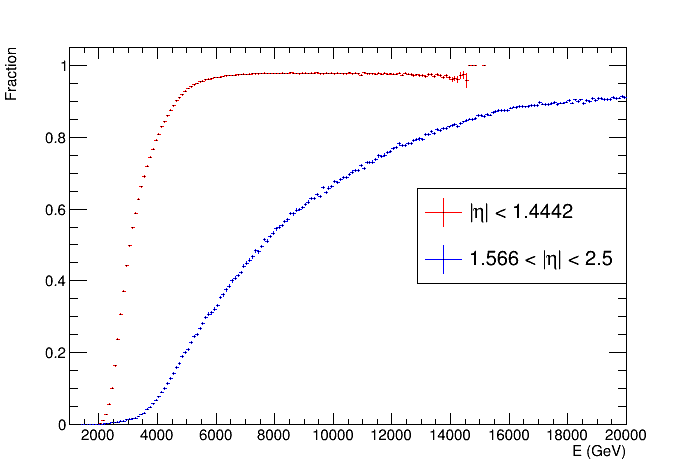
\includegraphics[width=0.9\textwidth]{chapters/Zprime/Saturation/images/FlatPt/Sample_variables/Barrel_Endcap_fraction.png}
    \end{tabular}
    \caption{The saturated fraction versus true (or mc) energy of electron for barrel (red points) and endcap (blue points).}
    \label{fig:S_Fraction}
  \end{center}
\end{figure}

\begin{figure}[bh]
  \begin{center}
    \begin{tabular}{cc}
      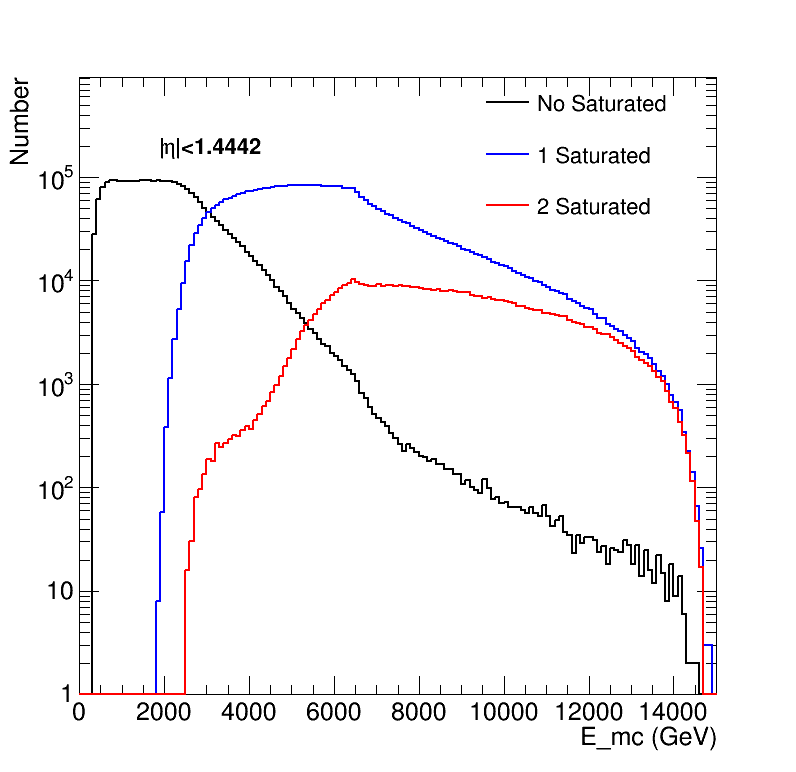
\includegraphics[width=0.45\textwidth]{chapters/Zprime/Saturation/images/FlatPt/Sample_variables/N_s_vs_Emc_Barrel.png} &
      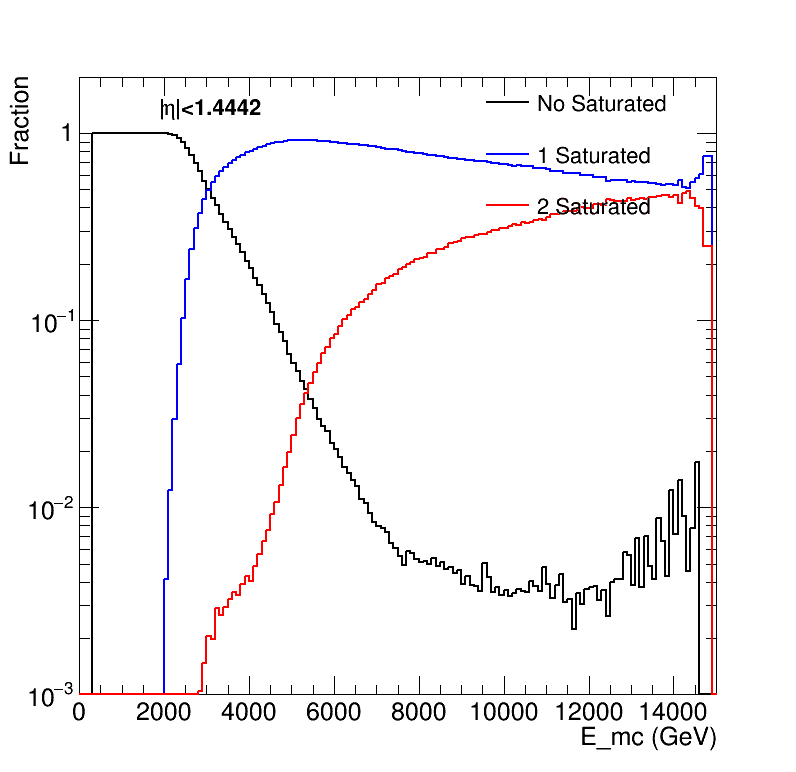
\includegraphics[width=0.45\textwidth]{chapters/Zprime/Saturation/images/FlatPt/Sample_variables/N_s_vs_Emc_fraBarrel.png} \\
      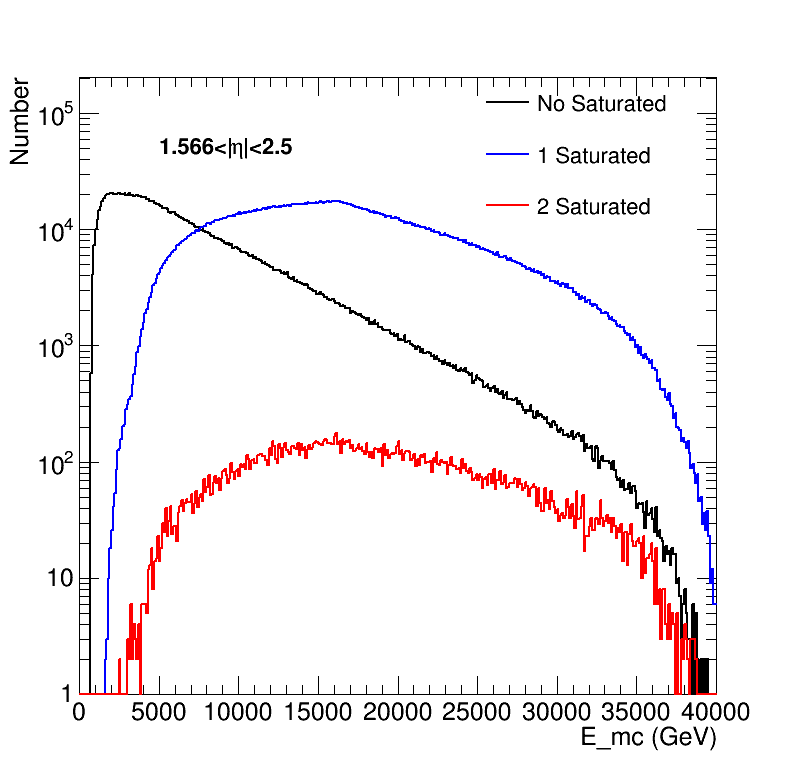
\includegraphics[width=0.45\textwidth]{chapters/Zprime/Saturation/images/FlatPt/Sample_variables/N_s_vs_Emc_Endcap.png} &
      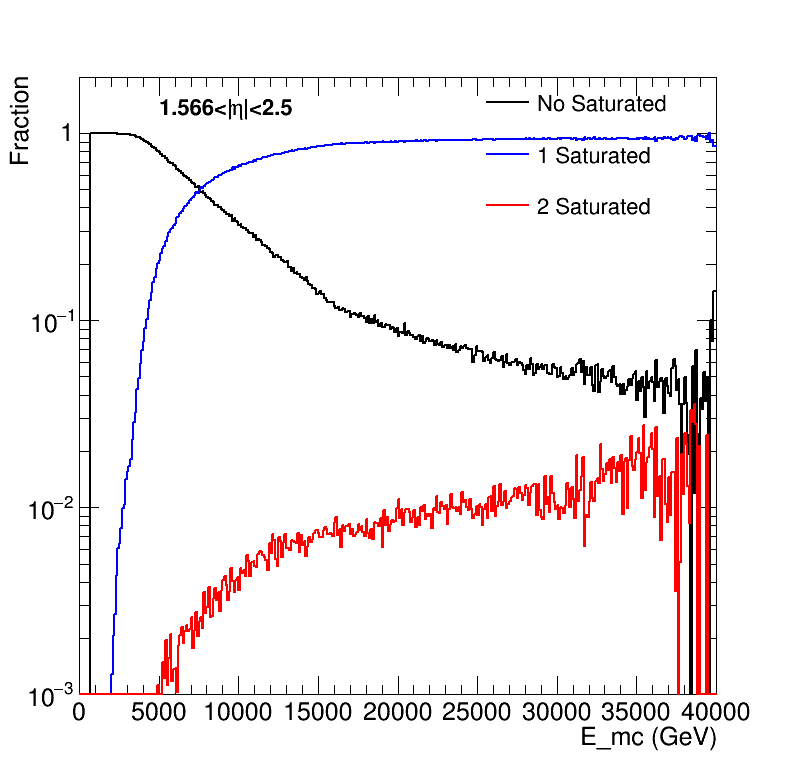
\includegraphics[width=0.45\textwidth]{chapters/Zprime/Saturation/images/FlatPt/Sample_variables/N_s_vs_Emc_fraEndcap.png} \\
    \end{tabular}
    \caption{The number of saturated crystals in $3\times3$ matrix with seed crystal in the center for different mc energy (left) and the fraction of number of saturated crystals in $3\times3$ matrix with seed crystal in the center for different mc energy (right) for barrel (top) and endcap (bottom).}
    \label{fig:N_S_Emc}
  \end{center}
\end{figure}

\subsubsection{Result}

The distribution of $(reco E - true E)/true E$ are shown in Figure \ref{fig:result_B_E} and one can see the energy of saturated electron from MVA is very close to true (or mc) energy. A fit to the MVA result using double-side CB is performed, the peak position and the standard deviation of the Gaussian core of the distributions are estimated through the fitted values of mean and sigma, respectively. The $'effective'$ standard deviation $\sigma_{eff}$, defined as half of the smallest interval around the peak position containing 68.3\% of the events, is used to assess the resolution, while taking into account possible non-Gaussian tails. We also checked the result by using MLP method which gives worse resolution shown in Figure \ref{fig:MLP_B_E} in section \ref{MLP_check}, therefore our basic method is BDTG method. Then we check the results for different $\eta$ which are shown in Figure \ref{fig:result_B123} and \ref{fig:result_E12}. From figures \ref{fig:result_B123} and \ref{fig:result_E12} we know the MVA works well for different $\eta$. Besides we check the MVA regressive results for different true energy of saturated electron which are shown in Figure \ref{fig:result_energy}. From Figure \ref{fig:result_energy} we see for barrel the results are stable for different energy, while for endcap the results are not very well in low energy, because for low electron energy the possibility of crystal to be saturated in endcap is very small and the training statistics for low energy and saturated electron is very less which can be seen in the bottom right plot of Figure \ref{fig:Ptmc_Emc_eta}.

\begin{figure}[bh]
  \begin{center}
    \begin{tabular}{cc}
      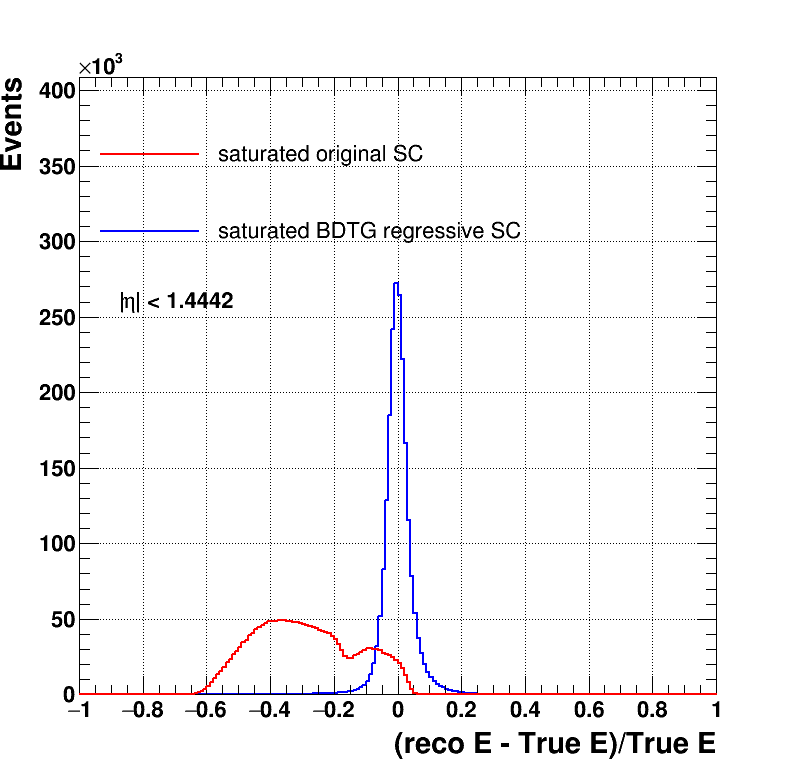
\includegraphics[width=0.45\textwidth]{chapters/Zprime/Saturation/images/FlatPt/Result/Barrel_Endcap/compare_BDTG_Barrel_Endcap_enSC_B_s.png} &
      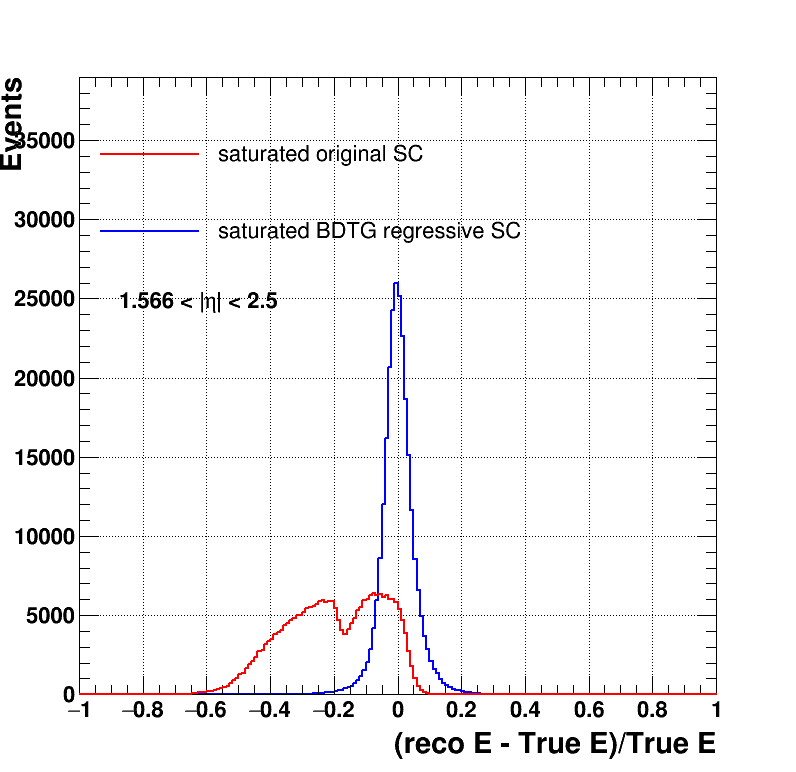
\includegraphics[width=0.45\textwidth]{chapters/Zprime/Saturation/images/FlatPt/Result/Barrel_Endcap/compare_BDTG_Barrel_Endcap_enSC_E_s.png} \\
      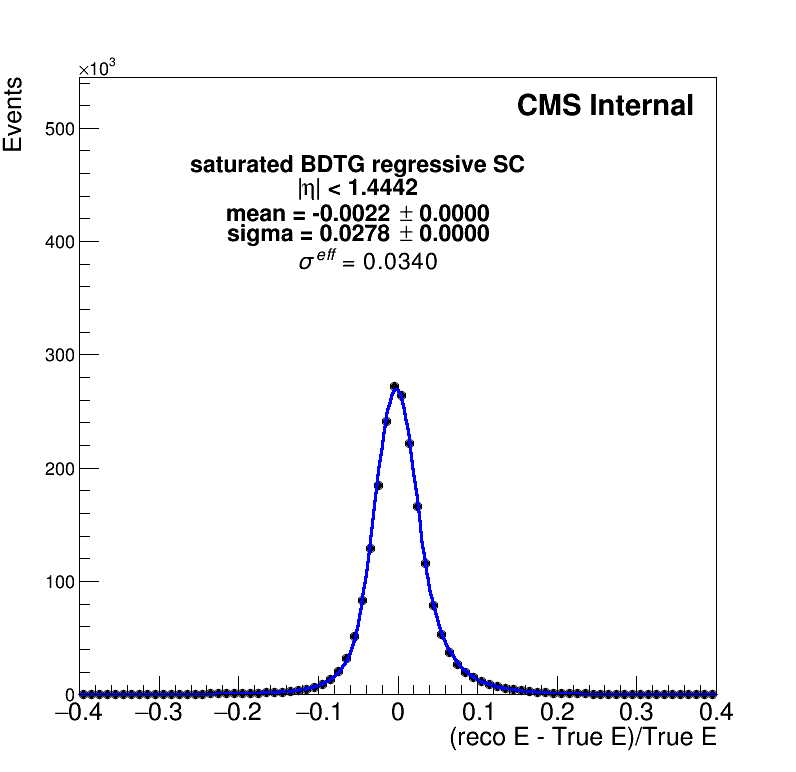
\includegraphics[width=0.45\textwidth]{chapters/Zprime/Saturation/images/FlatPt/Result/Barrel_Endcap/fit_BDTG_Barrel_Endcap_B_reg_s.png} &
      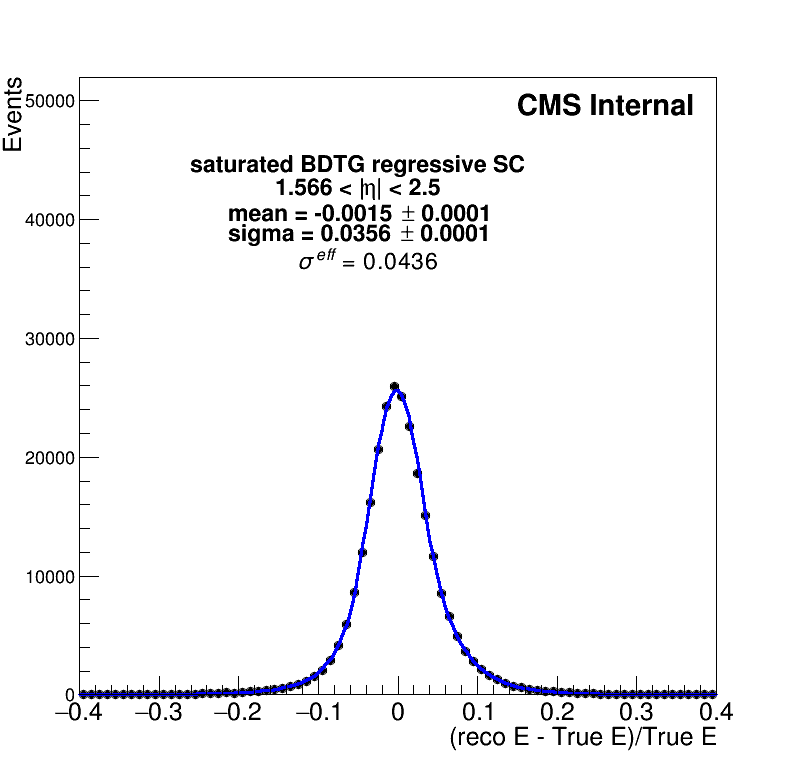
\includegraphics[width=0.45\textwidth]{chapters/Zprime/Saturation/images/FlatPt/Result/Barrel_Endcap/fit_BDTG_Barrel_Endcap_E_reg_s.png}
    \end{tabular}
    \caption{ The top plots are the distribution of supercluster energy minus ture energy divided by true energy for saturated electron for barrel (left) and endcap (right), the red histogram is for reconstructed supercluster enery, the blue histogram is for MVA regressive energy. The bottom plots are the fit of the blue histogram for barrel (left) and endcap (right).}
    \label{fig:result_B_E}
  \end{center}
\end{figure}



\begin{figure}[bh]
  \begin{center}
    \begin{tabular}{cc}
      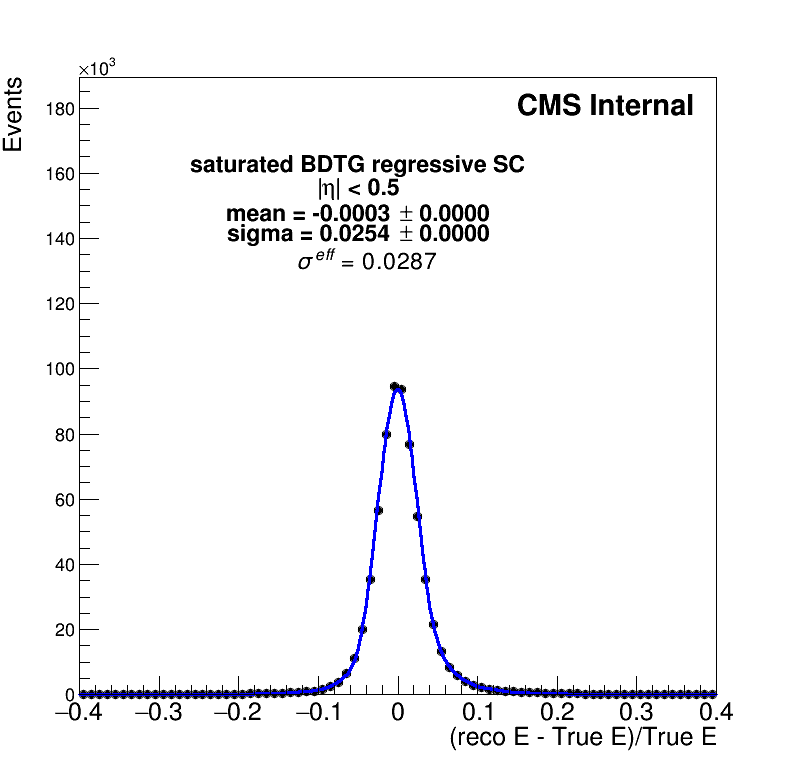
\includegraphics[width=0.45\textwidth]{chapters/Zprime/Saturation/images/FlatPt/Result/Barrel123_Endcap12/fit_BDTG_Barrel123_Endcap12_eta1_reg_s.png} &
      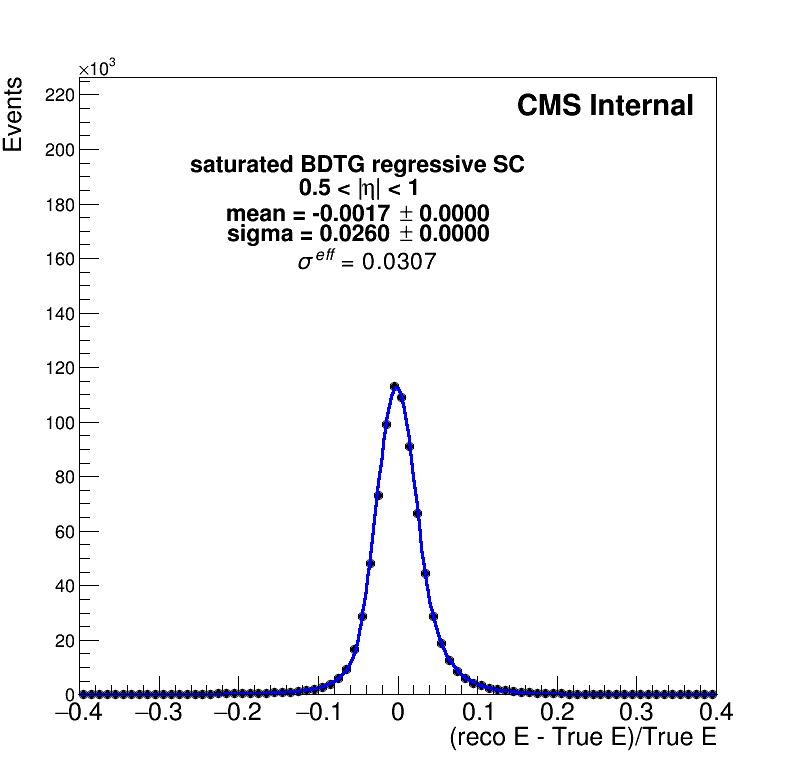
\includegraphics[width=0.45\textwidth]{chapters/Zprime/Saturation/images/FlatPt/Result/Barrel123_Endcap12/fit_BDTG_Barrel123_Endcap12_eta2_reg_s.png} \\
      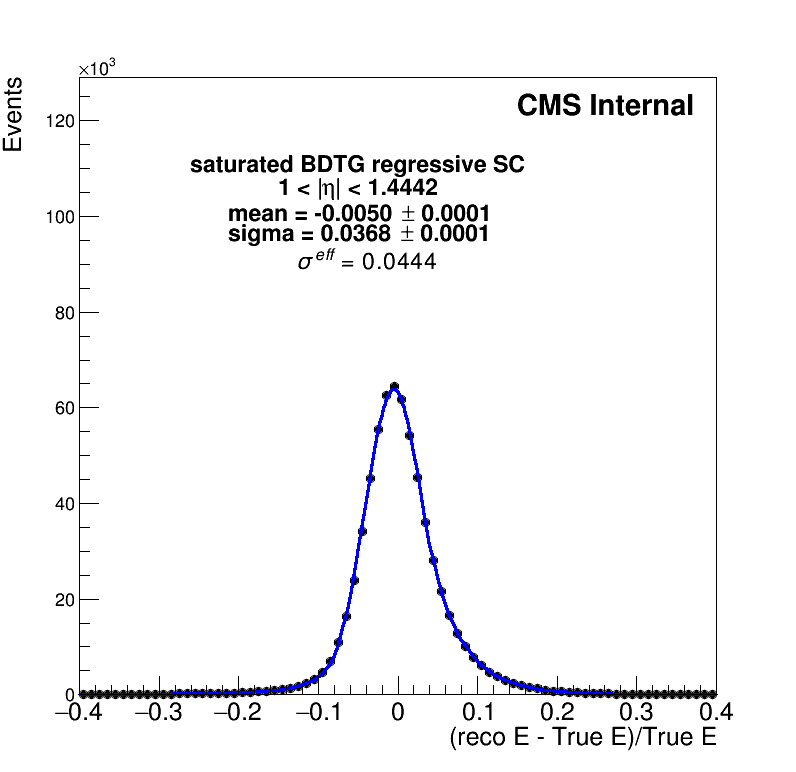
\includegraphics[width=0.45\textwidth]{chapters/Zprime/Saturation/images/FlatPt/Result/Barrel123_Endcap12/fit_BDTG_Barrel123_Endcap12_eta3_reg_s.png} &
    \end{tabular}
    \caption{ The distributions of MVA regressive energy minus ture energy divided by true energy for saturated electrons in barrel for different $\eta$ ranges.}
    \label{fig:result_B123}
  \end{center}
\end{figure}


\begin{figure}[bh]
  \begin{center}
    \begin{tabular}{cc}
      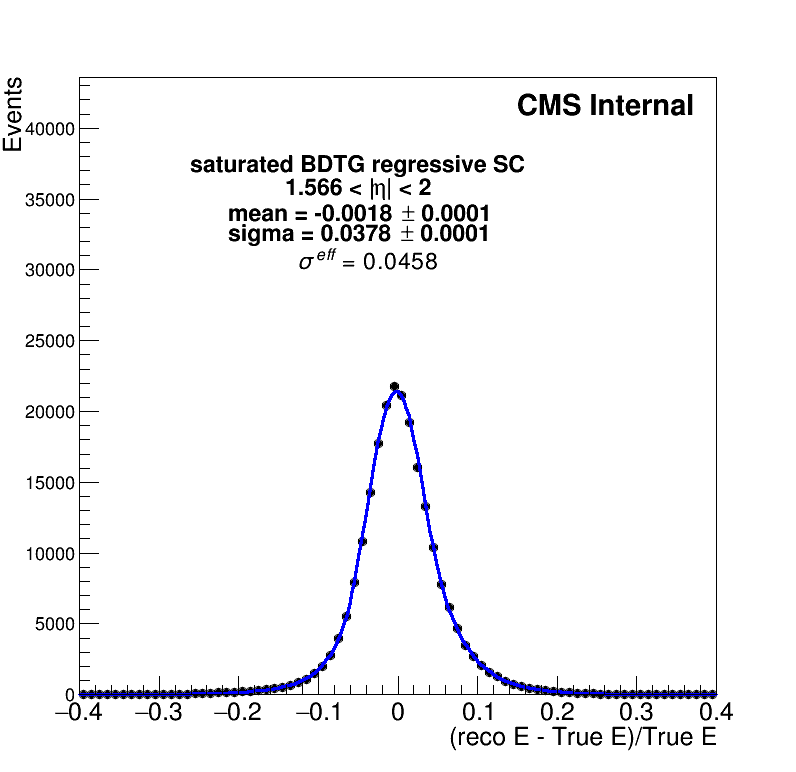
\includegraphics[width=0.45\textwidth]{chapters/Zprime/Saturation/images/FlatPt/Result/Barrel123_Endcap12/fit_BDTG_Barrel123_Endcap12_Eeta1_reg_s.png} &
      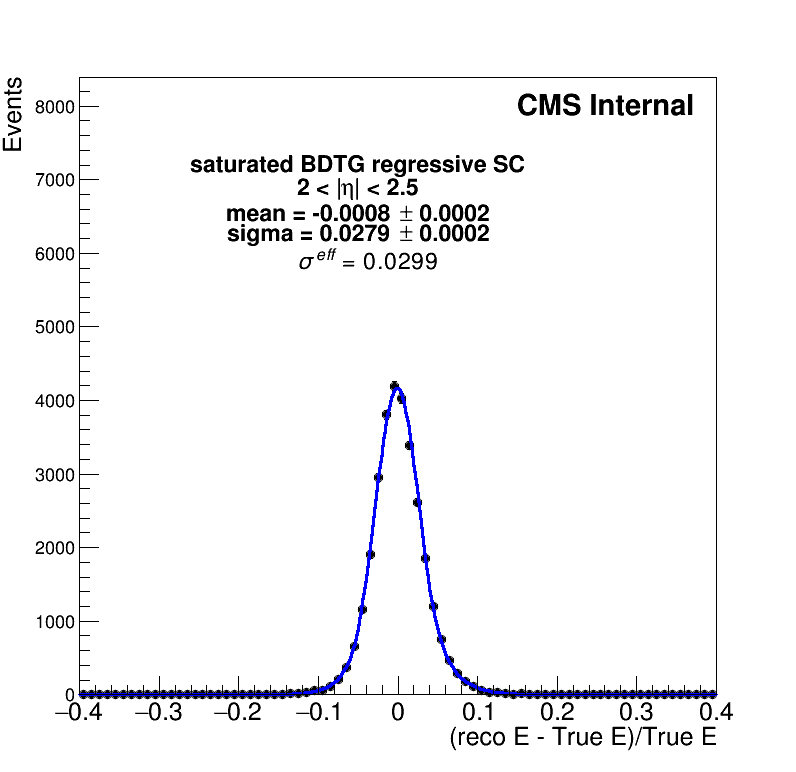
\includegraphics[width=0.45\textwidth]{chapters/Zprime/Saturation/images/FlatPt/Result/Barrel123_Endcap12/fit_BDTG_Barrel123_Endcap12_Eeta2_reg_s.png} \\
    \end{tabular}
    \caption{ The distributions of MVA regressive energy minus ture energy divided by true energy for saturated electron in endcap for different $\eta$ ranges.}
    \label{fig:result_E12}
  \end{center}
\end{figure}


\begin{figure}[bh]
  \begin{center}
    \begin{tabular}{cc}
      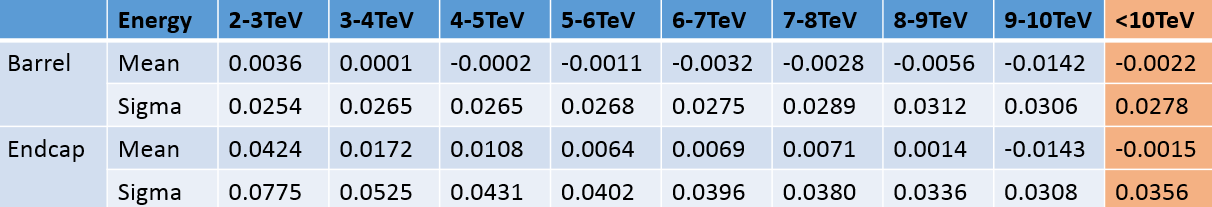
\includegraphics[width=0.9\textwidth]{chapters/Zprime/Saturation/images/FlatPt/Result/different_energy.png}
    \end{tabular}
    \caption{ The fit results for the distributions of MVA regressive energy minus ture energy divided by true energy for saturated electron for different true energy in barrel and endcap.}
    \label{fig:result_energy}
  \end{center}
\end{figure}

\subsubsection{Check the result in ZToEE samples}

Here we check the MVA result using ZToEE powheg sample with $M_{Z}$ great than 4500 GeV samples. The results are shown in figures \ref{fig:ZToEE_4500_6000_B_E} and \ref{fig:ZToEE_6000_Inf_B_E}. The result looks good.

\begin{figure}[bh]
  \begin{center}
    \begin{tabular}{cc}
      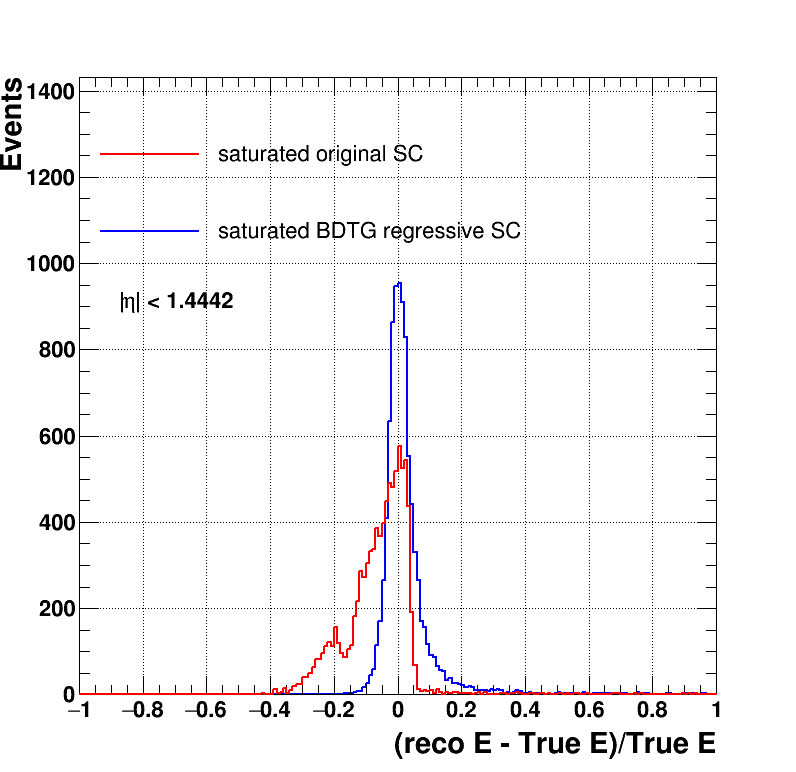
\includegraphics[width=0.45\textwidth]{chapters/Zprime/Saturation/images/FlatPt/ZToEE_check/4500_6000/compare_BDTG_Barrel_Endcap_enSC_B_s.png} &
      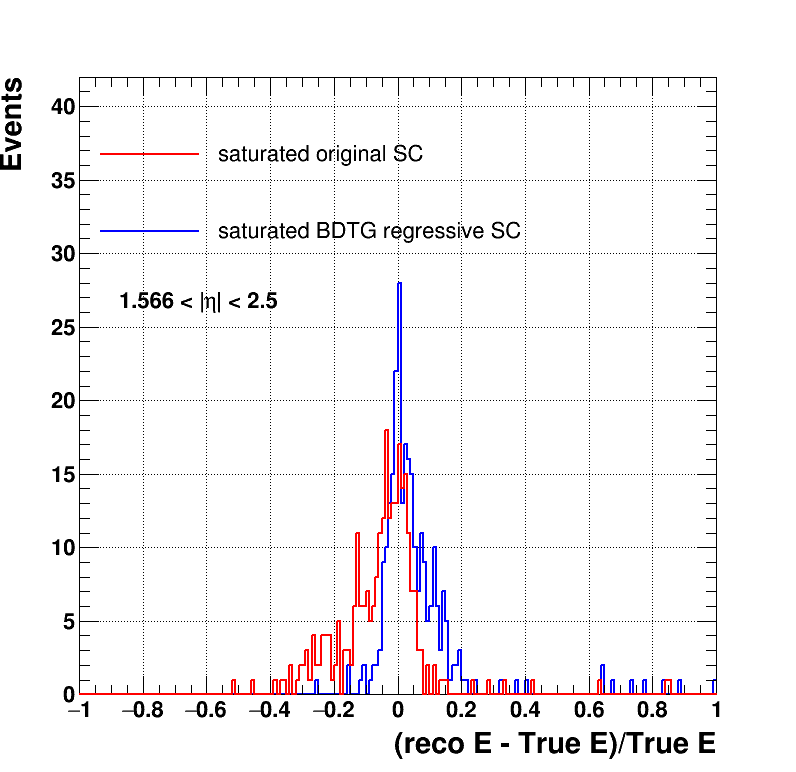
\includegraphics[width=0.45\textwidth]{chapters/Zprime/Saturation/images/FlatPt/ZToEE_check/4500_6000/compare_BDTG_Barrel_Endcap_enSC_E_s.png} \\
      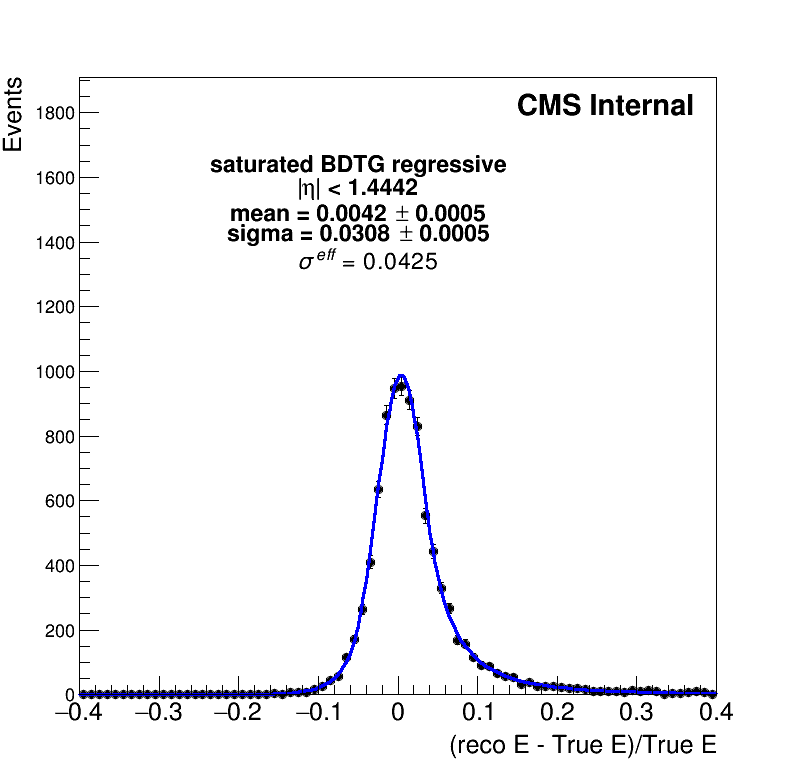
\includegraphics[width=0.45\textwidth]{chapters/Zprime/Saturation/images/FlatPt/ZToEE_check/4500_6000/fit_BDTG_Barrel_Endcap_B_reg_s.png} &
      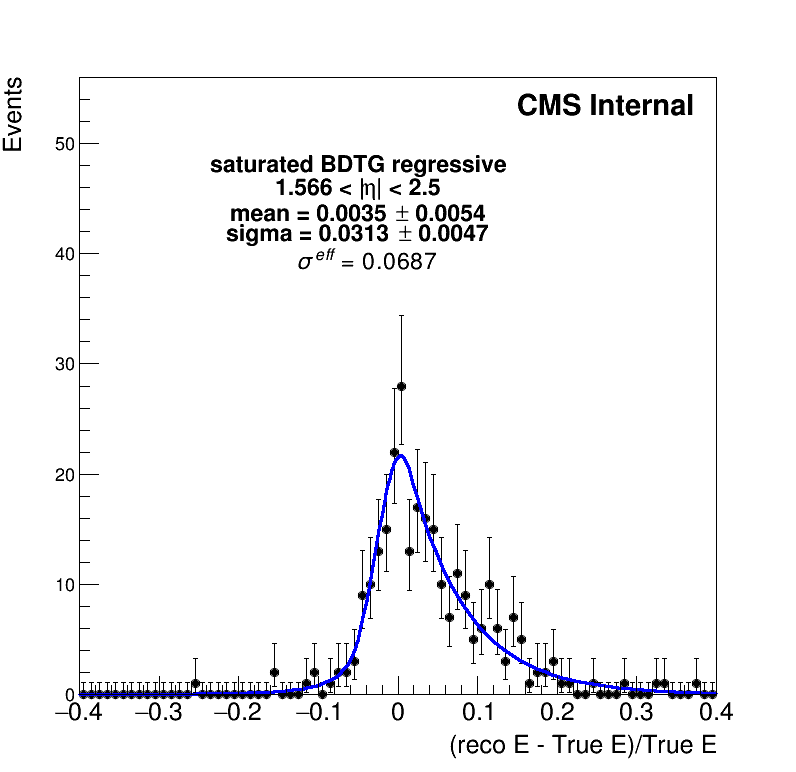
\includegraphics[width=0.45\textwidth]{chapters/Zprime/Saturation/images/FlatPt/ZToEE_check/4500_6000/fit_BDTG_Barrel_Endcap_E_reg_s.png}
    \end{tabular}
    \caption{ The top plots are the distribution of supercluster energy minus ture energy divided by true energy for saturated electron for barrel (left) and endcap (right) for ZToEE\_4500\_6000 sample, the red histogram is for reconstructed supercluster enery, the blue histogram is for MVA regressive energy. The bottom plots are the fit of the blue histogram for barrel (left) and endcap (right).}
    \label{fig:ZToEE_4500_6000_B_E}
  \end{center}
\end{figure}


\begin{figure}[bh]
  \begin{center}
    \begin{tabular}{cc}
      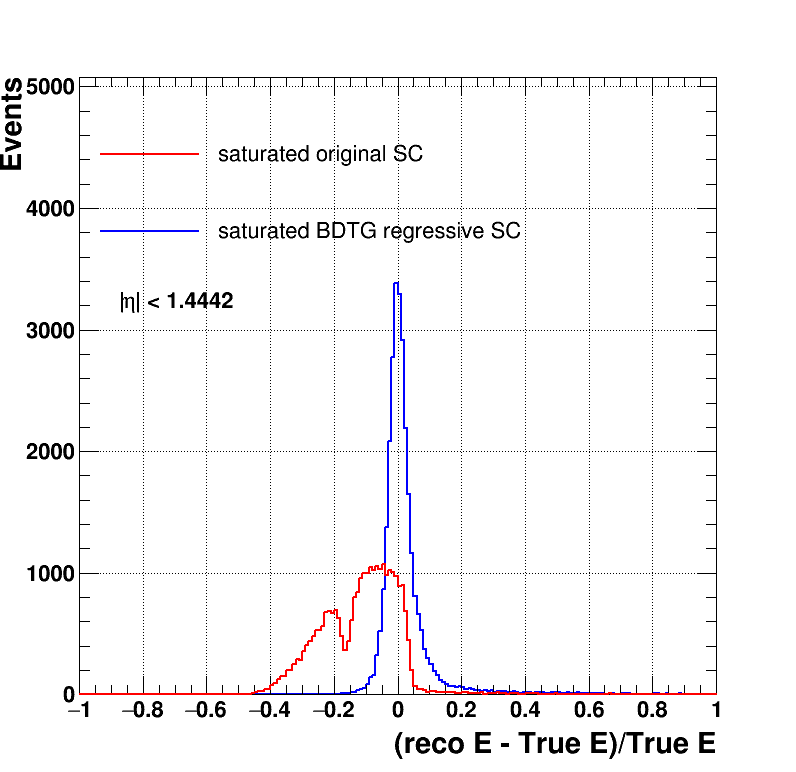
\includegraphics[width=0.45\textwidth]{chapters/Zprime/Saturation/images/FlatPt/ZToEE_check/6000_Inf/compare_BDTG_Barrel_Endcap_enSC_B_s.png} &
      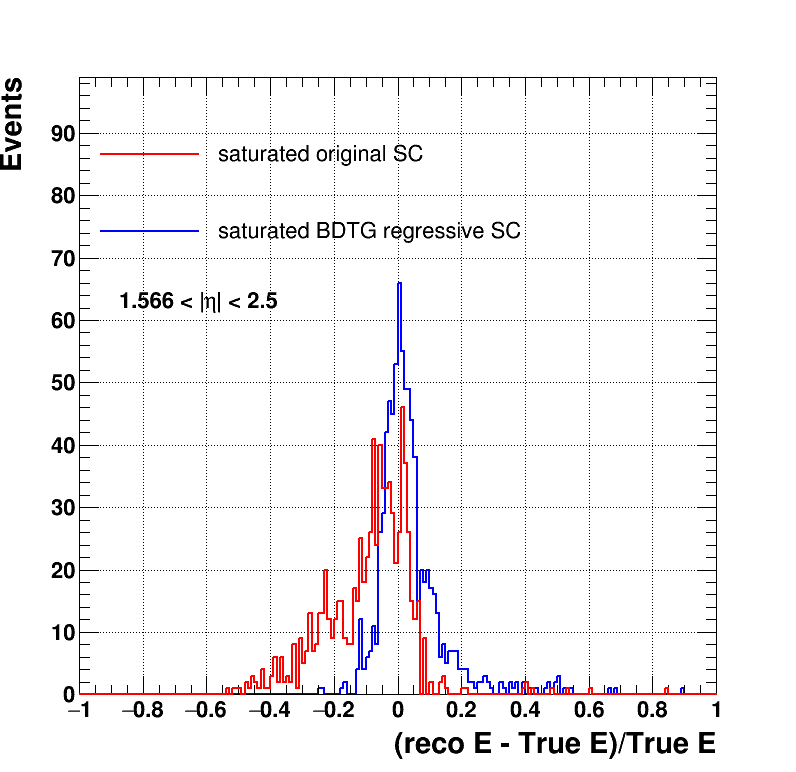
\includegraphics[width=0.45\textwidth]{chapters/Zprime/Saturation/images/FlatPt/ZToEE_check/6000_Inf/compare_BDTG_Barrel_Endcap_enSC_E_s.png} \\
      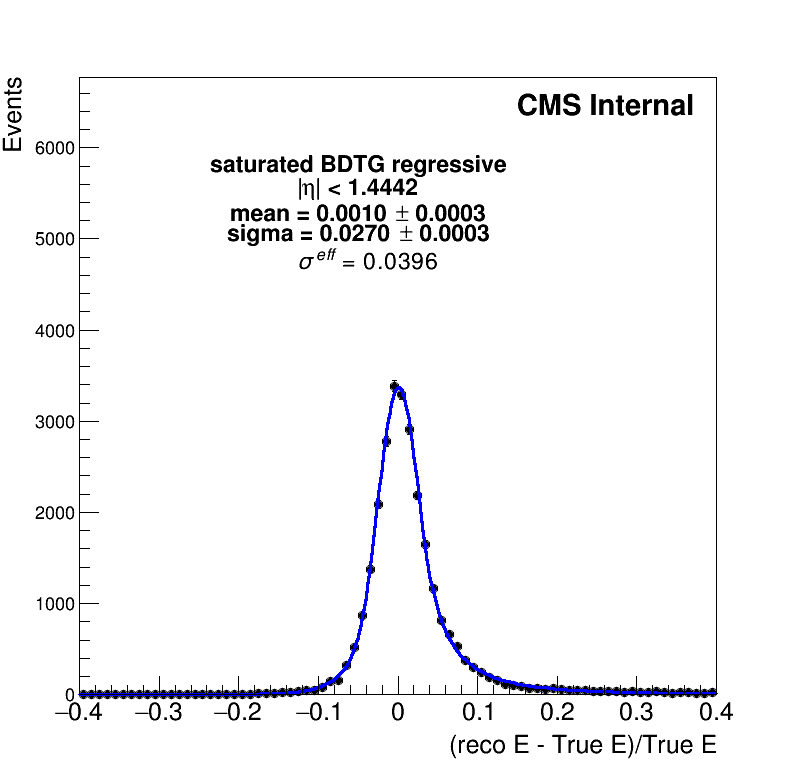
\includegraphics[width=0.45\textwidth]{chapters/Zprime/Saturation/images/FlatPt/ZToEE_check/6000_Inf/fit_BDTG_Barrel_Endcap_B_reg_s.png} &
      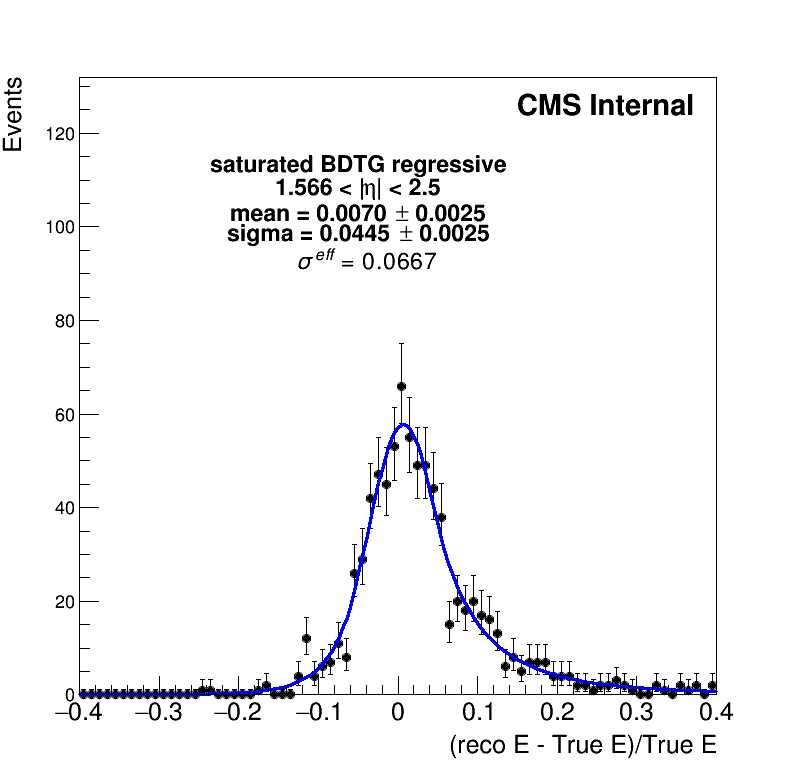
\includegraphics[width=0.45\textwidth]{chapters/Zprime/Saturation/images/FlatPt/ZToEE_check/6000_Inf/fit_BDTG_Barrel_Endcap_E_reg_s.png}
    \end{tabular}
    \caption{ The top plots are the distribution of supercluster energy minus ture energy divided by true energy for saturated electron for barrel (left) and endcap (right) for ZToEE$\_$6000$\_$Inf sample, the red histogram is for reconstructed supercluster enery, the blue histogram is for MVA regressive energy. The bottom plots are the fit of the blue histogram for barrel (left) and endcap (right).}
    \label{fig:ZToEE_6000_Inf_B_E}
  \end{center}
\end{figure}


\subsubsection{Apply to data}

Using DoubleEG dataset from 2016 in \ref{tab:Zprime-data-samples}, we find three events in which there are and only one saturated HEEP (High Energy Electron Pairs) electron. The energy of SC and MVA regressived energy are shown in Table  \ref{tab:detail}. The events displays are shown in Figure \ref{fig:event_display}.

\begin{table}[!h]
  \begin{center}
\smallskip\noindent
\resizebox{\linewidth}{!}{%
    \begin{tabular}{lllll}
      \hline
                    & event number & $\eta$    & SC energy (GeV)  & Regressived energy (GeV)  \\
      \hline
      electron1     & 1076867675   & 1.21759 & 2370.34          & 2279.53                   \\
      electron2     & 897834686    & 1.56931 & 2954.7           & 3167.63                   \\
      electron3     & 400840829    & 1.1476  & 2048.81          & 3151.99                   \\
      \hline
    \end{tabular}}
    \caption{Detail of saturated HEEP electrons.}
    \label{tab:detail}
  \end{center}
\end{table}

\begin{figure}[bh]
  \begin{center}
    \begin{tabular}{cc}
      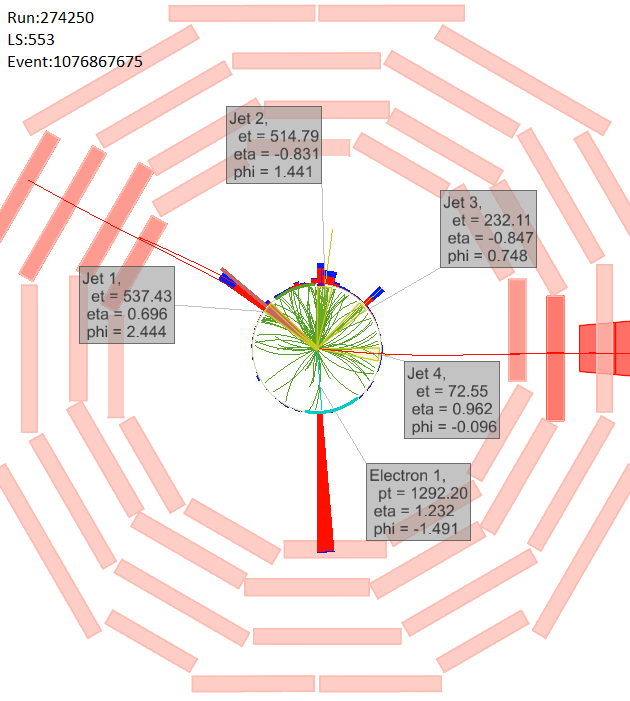
\includegraphics[width=0.45\textwidth]{chapters/Zprime/Saturation/images/FlatPt/cmsShow/274250_1076867675_553_RhoPhi.png} &
      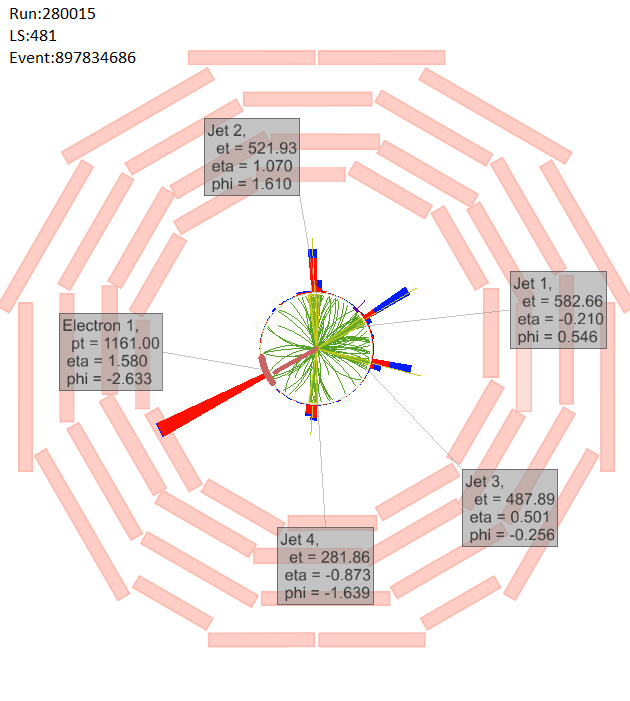
\includegraphics[width=0.45\textwidth]{chapters/Zprime/Saturation/images/FlatPt/cmsShow/280015_897834686_481_RhoPhi.png} \\
      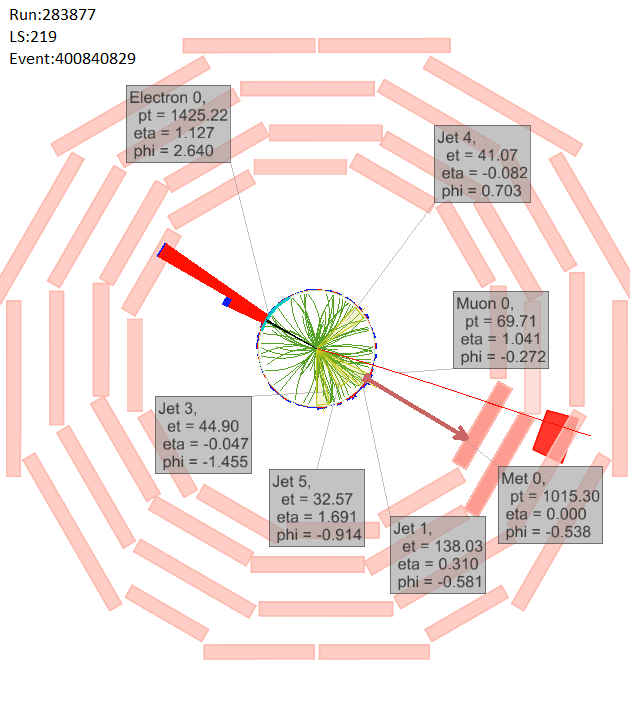
\includegraphics[width=0.45\textwidth]{chapters/Zprime/Saturation/images/FlatPt/cmsShow/283877_400840829_219_RhoPhi.png}
    \end{tabular}
    \caption{ The events displays of saturated HEEP electrons in data for $\rho\phi$ visual angle.}
    \label{fig:event_display}
  \end{center}
\end{figure}


\subsubsection{Prediction of saturated events}

The number of saturated DY events which contain saturated electron for $30~fb^{-1}$ luminosity is shown in Figure \ref{fig:Prediction_DY_s} and one can see the possibility to have one saturated DY event is $\sim 6\%$.

\begin{figure}[bh]
  \begin{center}
    \begin{tabular}{cc}
      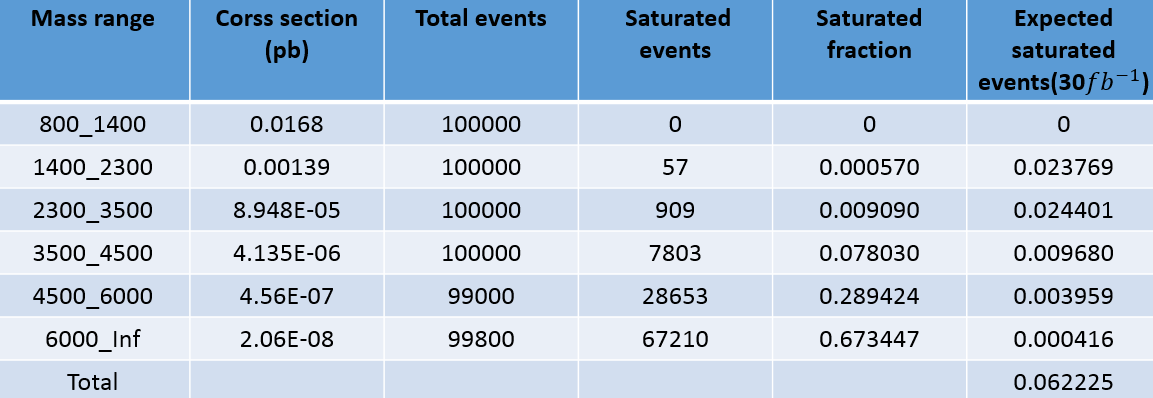
\includegraphics[width=0.9\textwidth]{chapters/Zprime/Saturation/images/FlatPt/Result/prediction.png} &
    \end{tabular}
    \caption{ The number of saturated DY events for $30~fb^{-1}$ luminosity.}
    \label{fig:Prediction_DY_s}
  \end{center}
\end{figure}
